\documentclass[tikz]{standalone}
\usepackage{pgfplots}
\pgfplotsset{compat=1.15}
\usepackage{mathrsfs}
\usetikzlibrary{arrows,calc}
\usepackage{tkz-euclide}

\pagestyle{empty}

\definecolor{AngleClr}{rgb}{0,0.39215686274509803,0}
\definecolor{ShapeClr}{rgb}{0.6,0.2,0}

\begin{document}

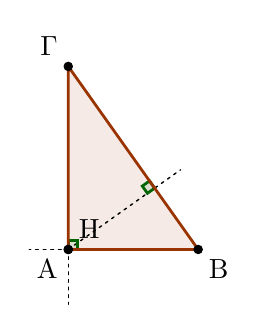
\begin{tikzpicture}[scale=.75]
\tkzSetUpLine[line width=1pt,color=black]
\tkzSetUpPoint[fill=black]

\tkzDefPoints{0/0/A,2.2/0/B,0/3.1/C}

\tkzDefTriangleCenter[ortho](A,B,C) \tkzGetPoint{H}

\tkzDefPointBy[projection=onto B--C](H)\tkzGetPoint{HA}

\tkzFillPolygon[fill=ShapeClr,fill opacity=0.1](A,B,C)

\tkzDrawSegments[line width=0.5pt,color=black,dashed,dash pattern=on 1pt off 1.75pt](H,A)

\tkzDrawSegments[line width=0.5pt,color=black,dashed,dash pattern=on 1pt off 1.75pt,add=0 and 0.3](B,A C,A A,HA)

\tkzMarkRightAngles[line width=1pt, size=.15,color=AngleClr,fill=AngleClr,fill opacity=0.1](C,A,B H,HA,C)
\tkzDrawPolygon[color=ShapeClr](A,B,C)



\tkzDrawPoints[size=3](A,B,C,H)
\tkzLabelPoint[below left](A){$\rm A$}
\tkzLabelPoint[below right](B){$\rm B$}
\tkzLabelPoint[above left](C){$\rm \Gamma$}

\tkzLabelPoint[above right](H){$\rm H$}

\end{tikzpicture}

\end{document}
